
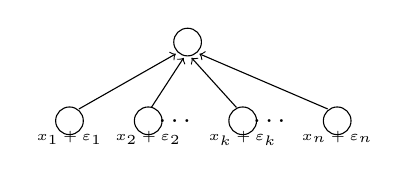
\begin{tikzpicture}
	\begin{scope}[every node/.style={sloped,allow upside down}]
		\draw (1.5,3) circle (0.5em);
		\draw (0,2) circle (0.5em)
		node[below=0.15] {\tiny $x_1 + \varepsilon_1$};
		\draw (1,2) circle (0.5em)
		node[below=0.15] {\tiny $x_2 + \varepsilon_2$}
		node[right=0.19] {\dots};
		\draw (2.2,2) circle (0.5em)
		node[below=0.15] {\tiny $x_k + \varepsilon_k$}
		node[right=0.19] {\dots};
		\draw (3.4,2) circle (0.5em) node[below=0.15] {\tiny $x_n + \varepsilon_n$};
		\draw[->] (0.12,2.15) -- (1.35,2.85);
		\draw[->] (1.04,2.17) -- (1.45,2.8);
		\draw[->] (2.12,2.17) -- (1.55,2.8);
		\draw[->] (3.28,2.15) -- (1.65,2.85);
	\end{scope}
\end{tikzpicture}
